\section{Counters, Decoders, and Segment Displays}
\label{lab_counters}

%\makelabheader %(Space for student name, etc., defined in master.tex)

\bigskip

\begin{enumerate}[wide]

\item Your kit contains several 7-segment displays for displaying numbers.  Find one of them with the characters ``M72'' on the side; this is the MAN72A, shown below.  Each of the 7 LEDs on its face has its anode (negative terminal) connected to one of the labeled inputs (A, B, C, etc.), and its cathode (positive terminal) connected to pin 14 and pin 3.  (Use either 14 or 3 for the connection; one is sufficient.) This configuration is called a ``common cathode'' arrangement, since all seven segments share the same positive terminal.  What number would the display show as it is wired below? 
\begin{center}
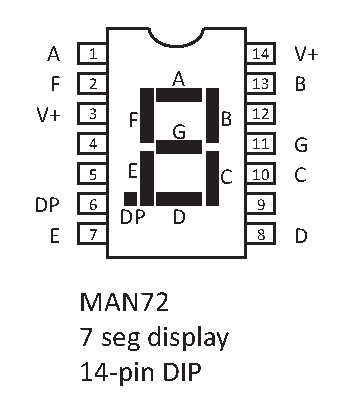
\includegraphics[scale=0.8]{appendices/pinouts/man72.eps}
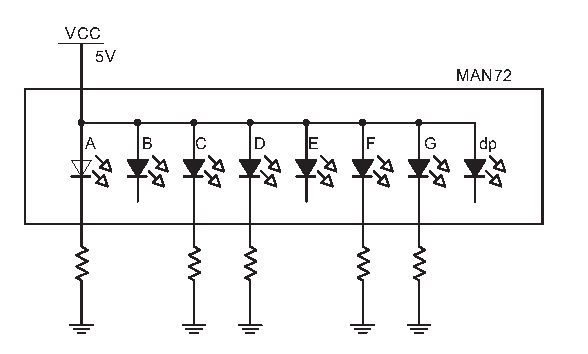
\includegraphics{counters/man72_circuit.eps}
\end{center}
  
\item A current of about 10~mA is required to make each segment light up brightly.  \textit{To limit the current, you will need to connect each anode to ground through an external resistor as shown in the diagram.  If you hook any of the segments directly between 5 volt supply and ground without a resistor, the display will get blown out.  (They're diodes, after all; each is only supposed to have a forward voltage of about 1.8 volts.)}  What value of resistor do you need to limit the current to 10~mA?)  Draw a circuit showing expressly how to light the ``B'' and ``C'' bars for the number 1.  Test your circuit, and verify that the current is what you think it is.  By the way, which two leads on your chip control the left and right decimal points? \label{part_man72_connections}

\end{enumerate}
\begin{enumerate}[wide,resume]


\begin{minipage}{.70\textwidth}

\item Suppose you have a series of digital signals that represent a binary number, as you did when you made a 2-bit adder.  (Recall that you had 3 output leads, representing the 1's, 2's, and 4's places.) Hooking up the 7-segment display directly to the output from your adder would be a royal pain; you'd need a LOT of logic gates to control which segments get illuminated for each of the possible combinations of output bits!  Fortunately, you have a chip that does this for you: the 74LS47.  The four binary inputs of the 74LS47 (A,B,C,D) represent the 1's, 2's, 4's, and 8's places, respectively.  Its 7 outputs (a,b,c,d,e,f,g) are designed to control the 7 LEDs on the MAN72 display; the 74L47 makes and breaks connections between each of those outputs and ground according to what number should be displayed.  Connect the 74LS47 inputs to logic switches, and connect the 74LS47 outputs to your MAN72 using resistors as you did in part~\ref{part_man72_connections}.  Connect pins 8 and 16 to ground and +5~V.  Pins 4, 5, and 6 should also be connected to 5~V for now.   Does the 74LS47 behave as you expect?  What happens when you give it a binary number greater than 9?  (NOTE: Remember what you discovered in Lab~\ref{lab_digital_electronics} part~\ref{part_open_digital_inputs}: any unused digital input A, B, C, or D has to be grounded; you can't just leave them hanging open.)  
\end{minipage}
\begin{minipage}{.28\textwidth}
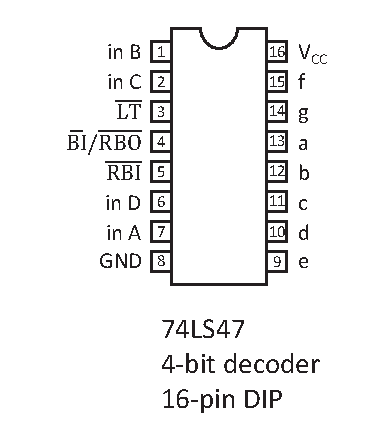
\includegraphics[scale=0.8]{appendices/pinouts/74LS47.eps}
\end{minipage}


\item What happens when you ground the input $\mathrm{\overline{LT}}$?  What about when you ground the input $\mathrm{\overline{BI}}$?  The bar over the letter means ``not''; in other words, whatever thing ``LT'' stands for will happen when that input is FALSE (0 volts) as opposed to when it's TRUE (5 volts).  By the way, consult the datasheet for the 74LS47: what \textit{does} ``LT'' stand for?

\item For comparison, the MAN74A, which is a ``common anode'' configuration, is shown below, as it would be wired to display one possible number.  Could you use the 74LS47 chip with the MAN74A?  (If yes, then build a circuit and show how.  If no, then explain why not.)
\begin{center}
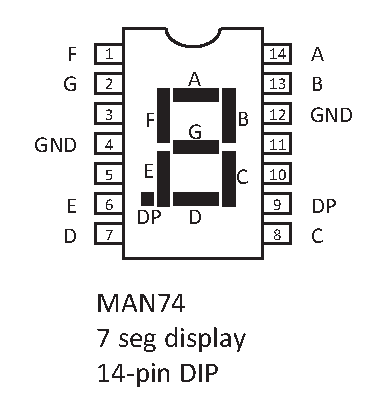
\includegraphics[scale=0.8]{appendices/pinouts/man74.eps}
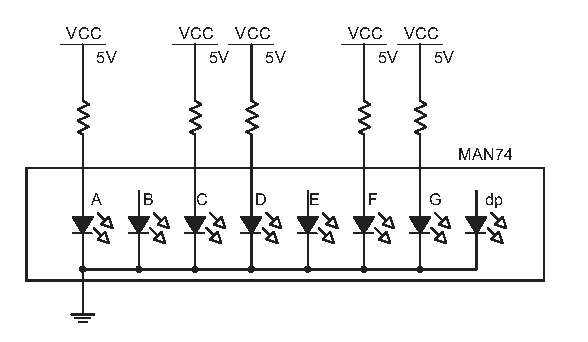
\includegraphics{counters/man74_circuit.eps}
\end{center}

\item Your kits contain another chip that counts: the CD74HC390E, whose pin-out is shown here.  Connect Vcc to +5 volts, and GND to ground.  Connect pin 4, labeled $1\mathrm{\overline{CP1}}$, to the TTL output of your function generator at 1~Hz.  Connect the outputs 1Q$_1$, 1Q$_2$, and 1Q$_3$ to three logic indicators on your breadboards.  The input 1MR should also be grounded.  How high does this chip count (in binary) when it is wired in this configuration?  

\vspace{-0.2in}
\begin{center}
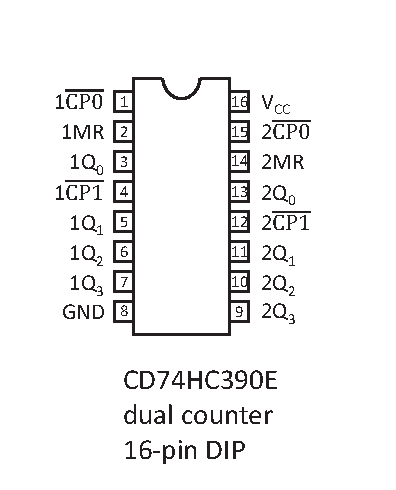
\includegraphics[scale=0.8]{appendices/pinouts/cd74hc390e.eps}
\end{center}
\vspace{-0.1in}

\item What happens when you disconnect the input 1MR (called the ``master reset'')?  What happens when you connect 1MR to +5 volts?

\item What condition at the clock input $1\mathrm{\overline{CP1}}$ is required to make the counter increment?  (A rising signal?  A falling signal?)

\item Now connect the TTL output of your function generator to the clock input $1\mathrm{\overline{CP0}}$, and connect the output 1Q$_0$ to the clock input $1\mathrm{\overline{CP1}}$.  Use your logic indicators to monitor all four outputs, 1Q$_0$ through 1Q$_3$.  How high does the chip count in this configuration?  

\item Predict what will happen if you change the configuration of the previous part so that the master reset 1MR is connected to the output 1Q$_3$.  How high will the chip count?  Test your prediction.

\pagebreak[2]
\item Perhaps you've noticed that your counter has a whole second set of inputs and outputs on the other side.  Show how you can hook up one of the outputs of the first set to one of the clock inputs of the second set to count from 0 to 99.  Connect each set of outputs to a 74LS47 decoder, controlling a 7-segment display.  Cool, huh?

\item How can you modify your counter to count from 0 to 39?  

\item What's the highest you could count to if you had three CD74HC390E chips?


\end{enumerate}
